
\chapter{Conceitos introdutórios de filtros}
\label{chap: introducao_filtros}

A medição de grandezas físicas é um aspecto fundamental no processo de decisão de autores autônomos, desde do ambiente hospitalar, onde os profissionais da saúde analisam sinais vitais dos pacientes, até em tarefas de exploração de planetas usando robôs, onde os sensores fornecem informações sobre o ambiente e o estado atual do robô. Em todos estes casos, a medição inerentemente envolve a presença de ruído, o que pode induzir diagnósticos errôneos da saúde do paciente ou acidentes com o robô. É comum que o sinal de interesse ocupe apenas uma determinada faixa de frequência e que os limites dela sejam conhecidos, dessa forma, o efeito do ruído pode ser mitigado se eliminarmos as componentes de frequências do sinal medido que estão fora da faixa de interesse a partir do uso de filtros eletrônicos.

\section{Categorização de filtros}

O filtro eletrônico é um circuito eletrônico que tem como função eliminar (reduzir) componentes de frequência indesejados, amplificar desejados, ou ambos. Ele pode ser caracterizado pela sua função de transferência,

\begin{equation}
    H(s) = \frac{V_{\text{out}}(s)}{V_{\text{in}}(s)},
\end{equation}
onde $V_{\text{in}}(s)$ e $V_{\text{out}}(s)$ são as tensões de entrada e saída do filtro, respectivamente.  

Avaliando $H(s)$ para $s = j\omega$, obtemos a função de transferência em frequência, a qual é um número complexo que pode ser descrito pelo seu módulo e fase,

\begin{equation}
    H(jw) = \| H(jw) \| e^{j\angle H(jw)},
\end{equation}
onde $\| H(jw) \|$ é o módulo e $\angle H(jw)$ é a fase. Em projeto de filtros, é comum que as especificações de ganho ou atenuação sejam dadas em decibéis. A função de Ganho $G(w)$ e a função de Atenuação $A(w)$ são definidas como:
\begin{equation}
    G(w) = 20 \log_{10} \| H(jw) \| (\text{dB}),
\end{equation}

\begin{equation}
    A(w) = -20 \log_{10} \| H(jw) \| (\text{dB}).
\end{equation}
Note que $G(w)$ e $A(w)$ são inversamente proporcionais e que $G(w) = -A(w)$. 


A partir da análise de $|H(jw)|$, podemos categorizar os filtros básicos como passa-baixas, passa-altas, passa-faixa, rejeita-faixa, e passa-tudo. A função básica de um filtro passa-baixas é atenuar as frequências acima de uma determinada frequência chamada de frequência de corte ($w_c$), enquanto realiza pouca ou nenhuma atenuação nas frequências abaixo de $w_c$. O filtro passa-altas, tem o comportamento inverso, ou seja, ele atenua as frequências abaixo de $w_c$ com pouca ou nenhuma atenuação nas as frequências acima de $w_c$. O filtro passa-faixa atenua as frequências fora de uma determinada faixa de frequência, enquanto o filtro rejeita-faixa atenua as frequências dentro de uma determinada faixa de frequência. O filtro passa-tudo, por sua vez, apresenta pouca ou nenhuma atenuação em todas as frequências. Cada um dos filtros são apresentados na figura~\ref{fig:filtros_basicos}.

\begin{figure}[h!]
    \centering
    \begin{minipage}[b]{0.32\linewidth}
        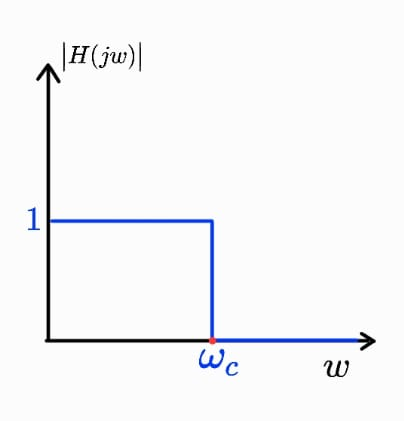
\includegraphics[width=\linewidth]{figuras/passa_baixa.png}
        \centering
        \\ \textbf{(a)}
    \end{minipage}
    \begin{minipage}[b]{0.32\linewidth}
        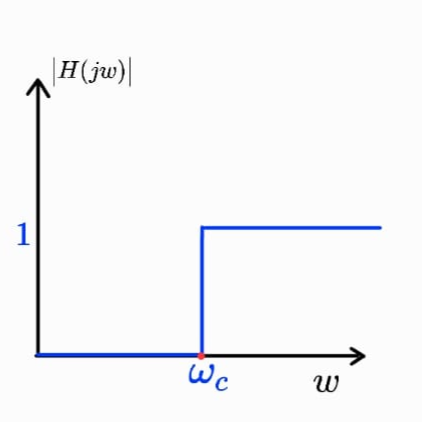
\includegraphics[width=\linewidth]{figuras/passa_altas.png}
        \centering
        \\ \textbf{(b)}
    \end{minipage}
    \begin{minipage}[b]{0.32\linewidth}     
        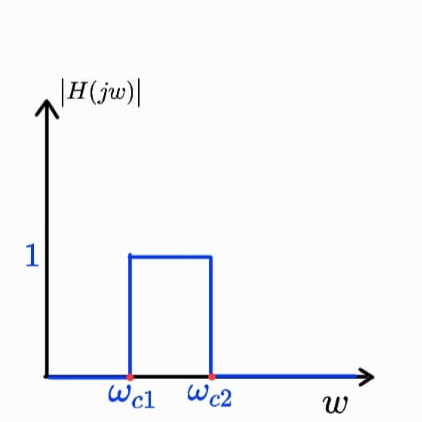
\includegraphics[width=\linewidth]{figuras/passa_faixa.png}
        \centering
        \\ \textbf{(c)}
    \end{minipage}
    \begin{minipage}[b]{0.32\linewidth}
        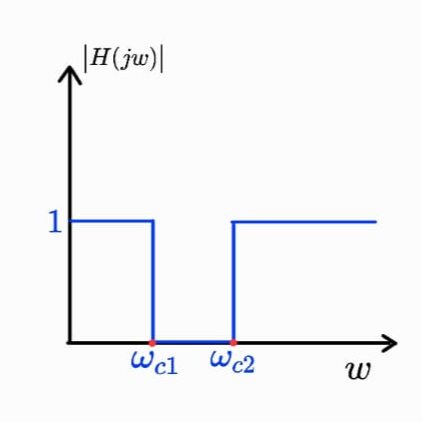
\includegraphics[width=\linewidth]{figuras/rejeita_faixa.png}
        \centering
        \\ \textbf{(d)}
    \end{minipage}
    \begin{minipage}[b]{0.32\linewidth}     
        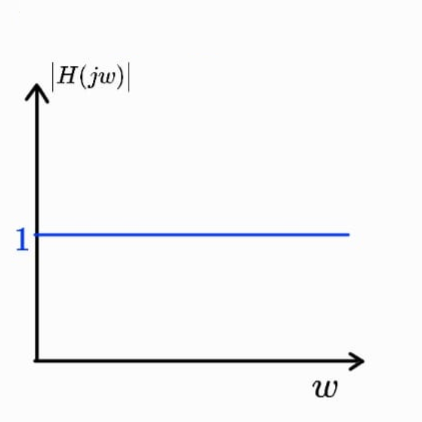
\includegraphics[width=\linewidth]{figuras/passa_tudo.png}
        \centering
        \\ \textbf{(e)}
    \end{minipage}
    \caption{Filtros básicos: (a) passa-baixa, (b) passa-alta, (c) passa-faixa, (d) rejeita-faixa e (e) passa-tudo.}
    \label{fig:filtros_basicos}
\end{figure}

A faixa de frequência em que o filtro apresenta pouca ou nenhuma atenuação é chamada de faixa de passagem, enquanto a faixa de frequência com atenuação significativa é chamada de faixa de rejeição. Uma das imperfeições dos filtros reais é que a transição entre a faixa de passagem e a faixa de rejeição não é abruta, mas sim graduação. A faixa que acontece essa transição é chamada de faixa de transição, tendo inicio na frequência $w_c$ e encerrando em uma frequência $w_s$, a qual é chamada de frequência de borda da faixa de rejeição. Outras imperfeições encontradas em filtros reais é que o filtro não atenua completamente ($\|H(w)\| > 0$) as frequências da faixa de rejeição e que ele apresenta atenuação $(\|H(w)\| < 1$) na faixa de passagem.

Diante das imperfeições dos filtros reais, é comum que além das especificações das frequências $w_c$ e $w_s$ também sejam especificações de projetos de filtros a atenuação máxima permitida na faixa de passagem $(A_{\text{max}})$ e atenuação mínima na faixa de rejeição $(A_{\text{min}})$. Essas especificações são ilustradas na figura~\ref{fig:filtros_reais} para os filtros passa-baixas, passa-altas, passa-faixa e rejeita-faixa. Note que as curvas em cada uma das faixas de frequência são apenas ilustrativas, pois a resposta em frequência de um filtro depende do projeto do mesmo. 

\begin{figure}[h!]
    \centering
    \begin{minipage}[b]{0.32\linewidth}
        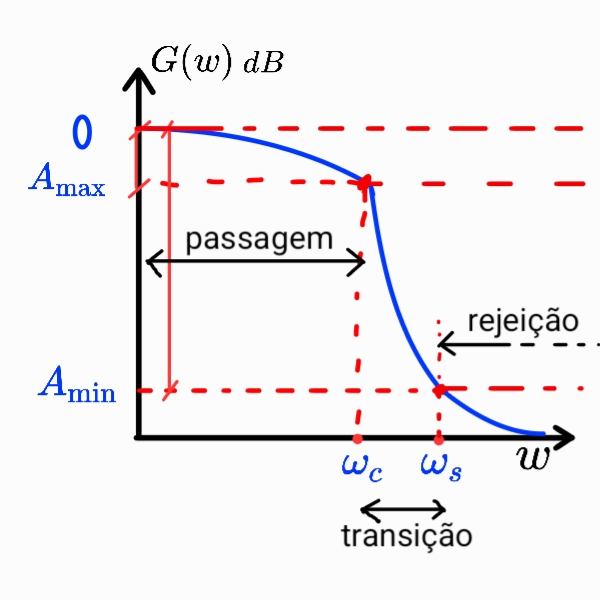
\includegraphics[width=\linewidth]{figuras/passa_baixas_real.png}
        \centering
        \\ \textbf{(a)}
    \end{minipage}
    \begin{minipage}[b]{0.32\linewidth}
        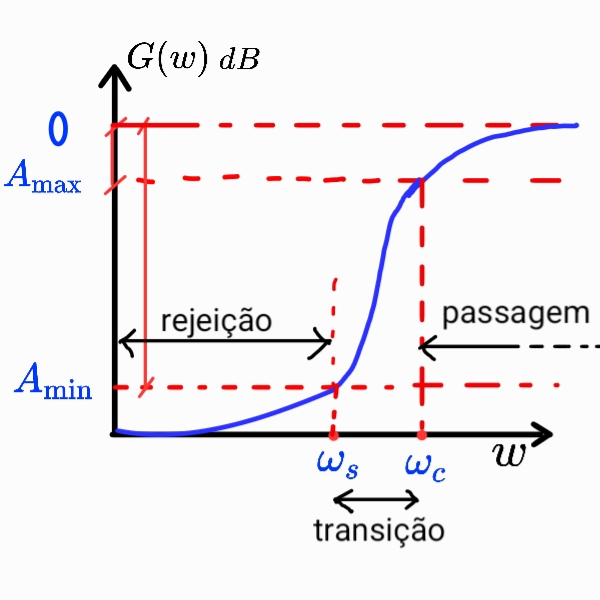
\includegraphics[width=\linewidth]{figuras/passa_altas_real.png}
        \centering
        \\ \textbf{(b)}
    \end{minipage}
    \\
    \begin{minipage}[b]{0.32\linewidth}     
        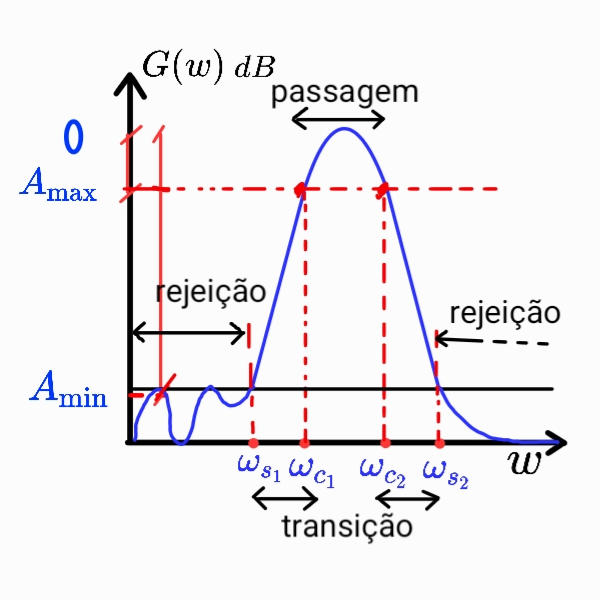
\includegraphics[width=\linewidth]{figuras/passa_faixa_real.png}
        \centering
        \\ \textbf{(c)}
    \end{minipage}
    \begin{minipage}[b]{0.32\linewidth}
        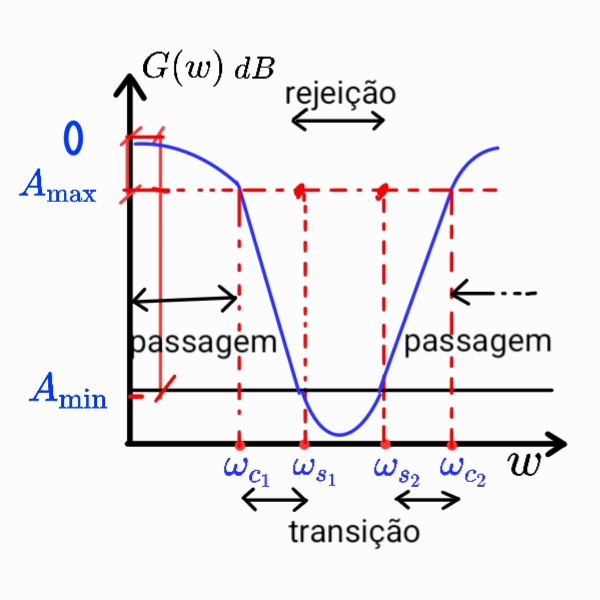
\includegraphics[width=\linewidth]{figuras/rejeita_faixa_real.png}
        \centering
        \\ \textbf{(d)}
    \end{minipage}
    \caption{Filtros básicos: (a) passa-baixa, (b) passa-alta, (c) passa-faixa, (d) rejeita-faixa.}
    \label{fig:filtros_reais}
\end{figure}

\section{Exemplos de filtros}

Na figura~\ref{fig:filtros_reais} estão apresentados exemplos circuitos de filtros passa-baixa, passa-alta e passa-faixa. As respostas em frequência desses circuitos são mostradas na figura~\ref{fig:LT_circuitos}.

\begin{figure}[h!]
    \centering
    \begin{minipage}[b]{0.32\linewidth}
        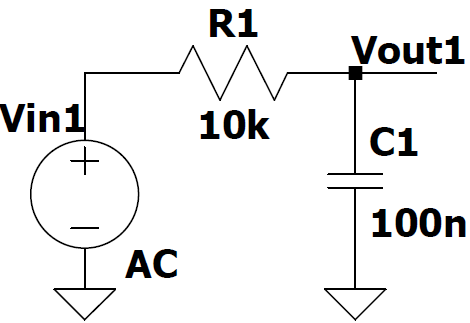
\includegraphics[width=\linewidth]{figuras/circuito_pb.png}
        \centering
        \\ \textbf{(a)}
    \end{minipage}
    \begin{minipage}[b]{0.32\linewidth}
        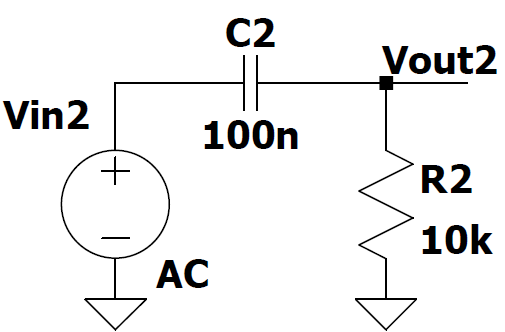
\includegraphics[width=\linewidth]{figuras/circuito_pa.png}
        \centering
        \\ \textbf{(b)}
    \end{minipage}
    \\
    \begin{minipage}[b]{0.49\linewidth}     
        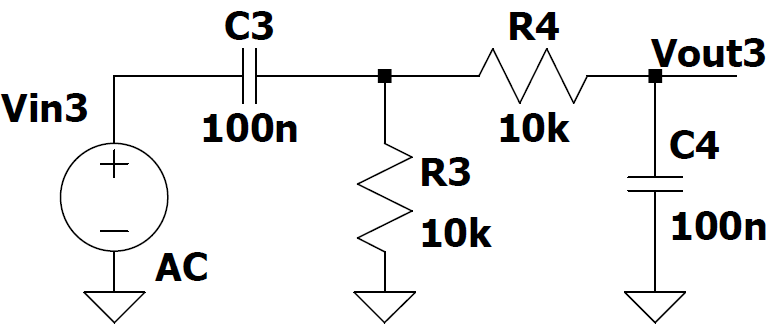
\includegraphics[width=\linewidth]{figuras/circuito_pf.png}
        \centering
        \\ \textbf{(c)}
    \end{minipage}
    %\begin{minipage}[b]{0.49\linewidth}
    %    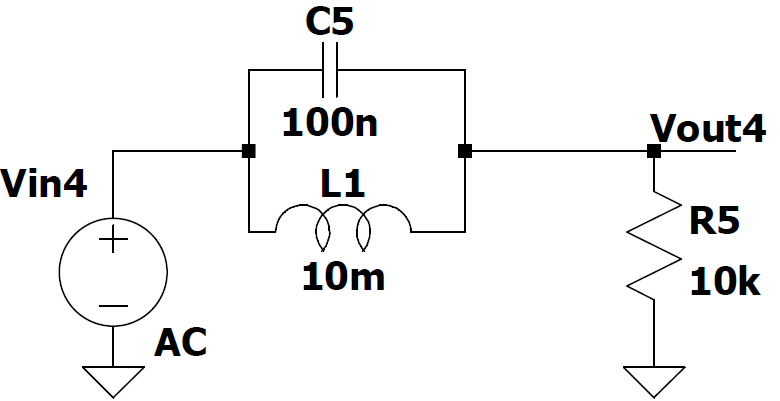
\includegraphics[width=\linewidth]{figuras/circuito_rf.png}
    %    \centering
    %    \\ \textbf{(d)}
    %\end{minipage}
    \caption{Exemplos de circuitos: (a) passa-baixa, (b) passa-alta, (c) passa-faixa.}
    \label{fig:filtros_reais}
\end{figure}

\begin{figure}[h!]
    \centering
    \begin{minipage}[b]{0.9\linewidth}
        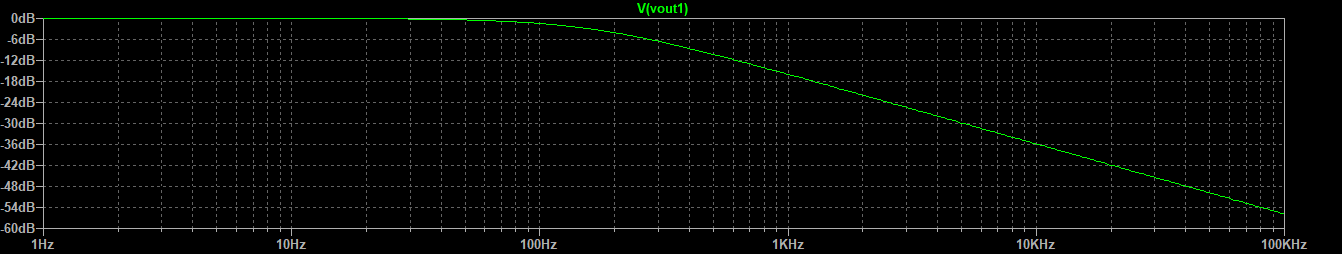
\includegraphics[width=\linewidth]{figuras/LT_pb.png}
        \centering
        \\ \textbf{(a)}
    \end{minipage}
    \begin{minipage}[b]{0.9\linewidth}
        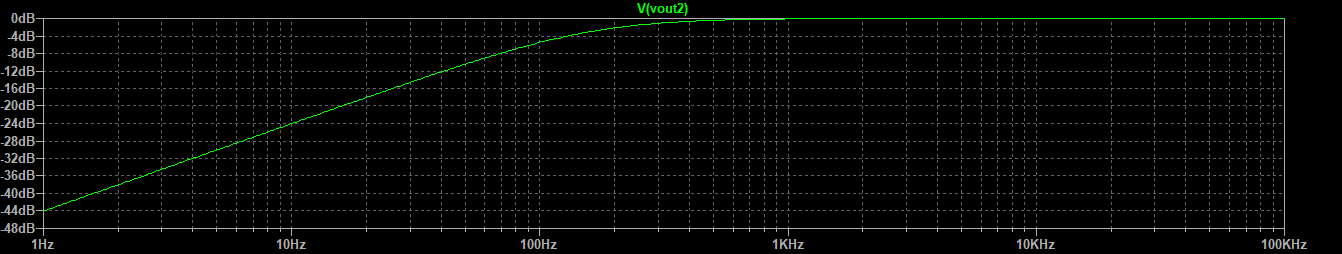
\includegraphics[width=\linewidth]{figuras/LT_pa.png}
        \centering
        \\ \textbf{(b)}
    \end{minipage}
    \begin{minipage}[b]{0.9\linewidth}     
        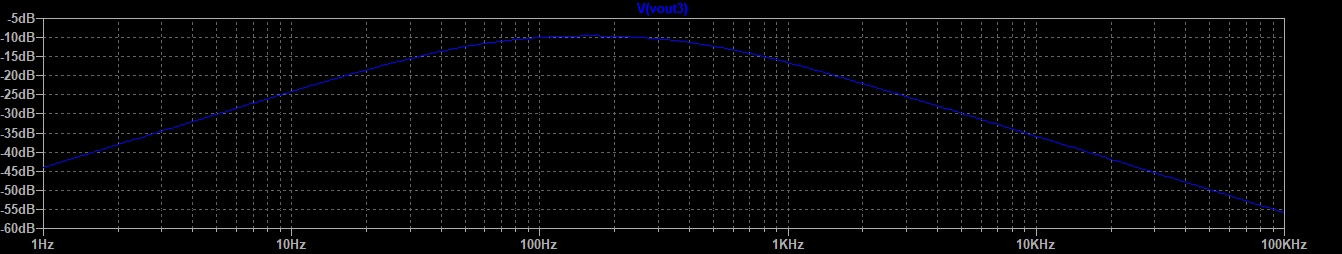
\includegraphics[width=\linewidth]{figuras/LT_pf.png}
        \centering
        \\ \textbf{(c)}
    \end{minipage}
    %\begin{minipage}[b]{0.9\linewidth}
    %    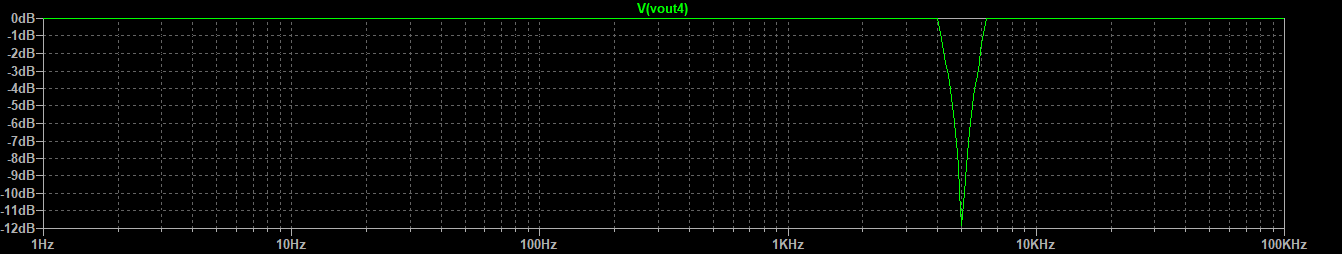
\includegraphics[width=\linewidth]{figuras/LT_rf.png}
    %    \centering
    %    \\ \textbf{(d)}
    %\end{minipage}
    \caption{Filtros básicos: (a) passa-baixa, (b) passa-alta, (c) passa-faixa.}
    \label{fig:LT_circuitos}
\end{figure}